% Bidirectional Heuristic Search on 3D Voxel Maps — AAAI 2027 (Camera-Ready).
% Overleaf: upload this folder (report.tex, aaai2027.sty, aaai2027.bst,
% references.bib) as a project; compile with pdfLaTeX. Minimal skeleton.

\documentclass[letterpaper]{article} % DO NOT CHANGE THIS
\usepackage{aaai2027}  % DO NOT CHANGE THIS
\usepackage[hyphens]{url}  % DO NOT CHANGE THIS
\usepackage{graphicx} % DO NOT CHANGE THIS
\urlstyle{rm} % DO NOT CHANGE THIS
\def\UrlFont{\rm}  % DO NOT CHANGE THIS
\usepackage{natbib}  % DO NOT CHANGE THIS AND DO NOT ADD ANY OPTIONS TO IT
\usepackage{caption} % DO NOT CHANGE THIS AND DO NOT ADD ANY OPTIONS TO IT
\frenchspacing  % DO NOT CHANGE THIS

\pdfinfo{
/TemplateVersion (2027.1)
}

\setcounter{secnumdepth}{0} % may set to 1 or 2 for numbered sections
\nocopyright               % removes the first-page copyright footnote

\title{Bidirectional Heuristic Search on 3D Voxel Maps}
\author{
    Gilad Shpigelman,
    Adam Rammal
}
\affiliations{
    Ben-Gurion University of the Negev\\
    Search Methods in Artificial Intelligence (237-2-5513) --- Advisor: Lior Siag
}

\begin{document}
\maketitle

\begin{abstract}
% Write last (~150 words): problem, method, headline result.
\end{abstract}

\section{Introduction and Literature Review}
% Background, motivation, problem statement; review of the theory papers.

\section{Methodology}
The contribution of this work is not the algorithms---they are established---but
\emph{how we measure them}: against a per-instance, provably minimal number of expansions.
We therefore describe the domain and algorithms only as far as reproducibility requires,
and develop the floor metric and the experiment built around it in full.

\subsection{Domain and Algorithms}
We use the Warthog 3D voxel benchmarks \citep{brewer2018voxel,nobes2023voxel}, running each
instance under two movement models: \textbf{26-connectivity}, where a voxel connects to all
$26$ neighbours at octile costs $\{1,\sqrt{2},\sqrt{3}\}$ under a \emph{no-corner-cutting}
rule (a diagonal step through a blocked voxel is illegal), and \textbf{6-connectivity},
the six axis-aligned neighbours at unit cost. The heuristic is the matching
coordinate-difference distance (3D octile, or Manhattan without diagonals). Crucially it is
\emph{consistent}: this is the precondition the must-expand theory below relies on
\citep{shaham2018consistent,siag2025bridging}, not an incidental detail.

We compare unidirectional \textbf{A*} \citep{hart1968astar} and its reverse against four
front-to-end bidirectional algorithms: \textbf{MM} \citep{holte2017mm}, ordering by
$\max(f,2g)$; \textbf{NBS} \citep{chen2017nbs}, near-optimal in expansions; \textbf{BAE*}
\citep{sadhukhan2013bae}, using the error estimate $b=f+d$; and \textbf{BiA*}, a Pohl-style
bidirectional A* \citep{pohl1971bidirectional} we implemented (it is absent from HOG2),
terminating when $U \le \max(f^{\min}_F, f^{\min}_B)$. \textbf{GBFS} serves as a fast,
suboptimal reference. Two points are not boilerplate: BiA* is our own code, and BAE*'s
lower bound rounds up to the greatest common divisor of the edge costs---unsound for the
irrational $\{\sqrt2,\sqrt3\}$ costs, so we disable that rounding to restore optimality.

\subsection{The Must-Expand Floor: Our Metric of Record}
Comparing raw expansion counts, or one algorithm against another, cannot say whether a
search was \emph{good in absolute terms}. So instead of a relative comparison we measure
every algorithm against the provable minimum number of expansions that \emph{any}
front-to-end bidirectional algorithm with the same heuristic must perform on that instance
\citep{eckerle2017sufficient,shaham2017minimal}. This floor is the backbone of the entire
study; the rest of the method exists to compute and exercise it correctly.

Fix an instance with optimal cost $C^\ast$, which we take from an exact A* solve---using the
\emph{recovered path length}, not the value stored in the scenario file, which is rounded
and would corrupt the strict comparisons below. A forward node $u$ is a must-expand
candidate iff $f_F(u) < C^\ast$, and symmetrically a backward node $v$ iff $f_B(v) < C^\ast$;
a pair $(u,v)$ forms a must-expand edge iff
\[
  g_F(u) + g_B(v) < C^\ast .
\]
Any algorithm must expand at least one endpoint of every such edge, so a \emph{vertex
cover} of this graph lower-bounds expansions, and the tightest bound is its minimum vertex
cover. For consistent heuristics the optimal cover has a threshold form
\citep{shaham2018consistent}, which turns an NP-hard problem into a linear scan:
\[
  |\mathrm{VC}| \;=\; \min_{\tau}\;\Big(\;\#\{u : g_F(u) < \tau\}
      \;+\; \#\{v : g_B(v) < C^\ast - \tau\}\;\Big).
\]
We recover the two $g$-value multisets by expanding each direction's full $f<C^\ast$ contour
(consistency makes the first settle of a node optimal), then scan $\tau$ over their
breakpoints for the minimum. Every result is reported as \textbf{expansions divided by this
floor}: a value of $1.0\times$ means the search was \emph{provably optimal}---it could not
have expanded fewer nodes---and larger values are the exact factor of avoidable work.

\subsection{The Heuristic-Strength Experiment}
The floor tells us how far each algorithm is from optimal at full heuristic strength; the
central \emph{question} of bidirectional search is when it becomes worthwhile at all. We
test this directly with a controlled weakening experiment. Our environment exposes a weight
$h'(\cdot)=w\,h(\cdot)$, $w\in[0,1]$: at $w{=}1$ the heuristic is the exact octile distance,
at $w{=}0$ the search degenerates to Dijkstra's algorithm, and every value in between
remains admissible. Holding the domain, instances, and algorithms fixed, we sweep $w$
downward and locate the crossover at which bidirectional search overtakes A*---a direct
test of the theory's claim that the bidirectional advantage is heuristic-dependent
\citep{alcazar2020unifying,siag2025bridging}.

\subsection{Setup, Correctness, and Reported Statistics}
The search core is HOG2 \citep{sturtevant2016hog2}, compiled headless for the cluster; on
top of it our voxel environment implements both move models, no-corner-cutting, the weight
knob, and the floor. We run three families of differing structure---\emph{industrial
plants} (cluttered), \emph{sandstone} (porous), and \emph{descent} (maze-like)---solving
each instance in both directions, every run isolated in a forked process under a wall-clock
timeout and a memory cap, dispatched as a Slurm array. Timeouts and failures are recorded,
never silently dropped.

Because we assert optimality, we verify it: an \emph{independent} auditor re-implements the
move rule from scratch and finds \textbf{0 illegal moves} across ${\sim}1.8$M generated
successors and ${\sim}58$k path edges, and all optimal algorithms agree on $C^\ast$.

``Comparing the algorithms'' is not a single number, and the literature we build on measures
several complementary things \citep{holte2017mm,alcazar2020unifying,siag2025bridging}. We
report each algorithm along the following axes:
\begin{itemize}
  \item \textbf{(A) Search efficiency}---expansions divided by the must-expand floor. This
  is the theory currency \citep{siag2025bridging} and our primary axis. We report the
  \emph{median} (not the mean: the distribution is heavy-tailed, so the mean tracks a few
  pathological instances), together with the per-instance \textbf{win rate}.
  \item \textbf{(B) Time efficiency}---wall-clock time and time-per-expansion. The latter
  separates search work (node count, axis A) from per-node overhead; we read wall-clock with
  care, as it reflects our implementation as well as the algorithm.
  \item \textbf{(C) Robustness}---the timeout and failure rate on hard instances, which also
  bounds the set of instances axis A is summarised over.
  \item \textbf{(D) Direction}---forward vs.\ backward search of the same instance, a
  first-class property of these benchmarks, whose authors document a directional bias in the
  maps themselves \citep{brewer2018voxel,nobes2023voxel}.
\end{itemize}
Axis \textbf{(E)}, the dependence of all of the above on \emph{heuristic strength}, is the
dedicated weakening experiment of the previous subsection. The organising question, following
\emph{bridging theory and practice} \citep{siag2025bridging}, is where an algorithm's
theoretical efficiency (A) does and does not translate into practical performance (B, C).

\section{Experimental Results}
We ran all seven algorithms on the three domains in both movement models and both
directions: plants (5 maps, 200 instances each), sandstone (11 maps, 25 each), and descent
(29 maps, 250 each). Optimality was consistent across every group---all optimal algorithms
returned identical costs on every solved instance, over ${\sim}64$k runs. We report along
the five axes of the previous section; values are medians over solved instances.

\subsection{(A) Distance from the floor}
Table~\ref{tab:expfloor} and Figure~\ref{fig:expfloor} give median expansions divided by the
must-expand floor. \textbf{Forward A* is essentially optimal} on all three domains---within
0--5\% of the provable minimum in every configuration---confirming that, with a strong
consistent heuristic, unidirectional search already expands nearly the minimal set. The
bidirectional algorithms pay a \textbf{2--5$\times$ premium}: BiA* is consistently cheapest
(${\sim}2\times$) and MM the most expensive. The gap is widest on the blocky plants and
narrower on the porous sandstone and maze-like descent.

\begin{table}[t]
\centering\small
\begin{tabular}{lcccccc}
\hline
domain / mode & A* & BiA* & NBS & BAE* & MM & rev-A* \\
\hline
plants · diag      & \textbf{1.00} & 2.00 & 2.21 & 3.78 & 5.12 & 4.64 \\
plants · nodiag    & \textbf{1.02} & 2.03 & 3.10 & 3.50 & 3.63 & 2.82 \\
sandstone · diag   & \textbf{1.00} & 1.98 & 2.01 & 2.41 & 2.75 & 2.69 \\
sandstone · nodiag & \textbf{1.05} & 2.01 & 2.38 & 2.63 & 2.96 & 2.51 \\
descent · diag     & \textbf{1.00} & 1.99 & 2.00 & 2.34 & 3.26 & 2.26 \\
descent · nodiag   & \textbf{1.01} & 2.00 & 2.21 & 2.75 & 3.11 & 2.48 \\
\hline
\end{tabular}
\caption{Median expansions / must-expand floor (1.0 = provably optimal).}
\label{tab:expfloor}
\end{table}

\begin{figure}[t]
\centering

\includegraphics[width=\columnwidth]{figures/exp_over_mvc.pdf}
\caption{Expansions relative to the theoretical minimum. A* sits on the floor; the
bidirectional methods sit above it.}
\label{fig:expfloor}
\end{figure}

Per instance (Figure~\ref{fig:winrate}), A* expands the fewest nodes on the large majority of
problems; among the bidirectional methods BiA* takes most of the remainder.

\begin{figure}[t]
\centering

\includegraphics[width=0.86\columnwidth]{figures/winrate.pdf}
\caption{Per-instance winner among the optimal algorithms.}
\label{fig:winrate}
\end{figure}

\subsection{(B) Time}
A* is also the fastest in wall-clock and MM the slowest. Dividing time by expansions isolates
per-node overhead: MM costs ${\sim}21\,\mu$s/expansion against ${\sim}2.5$--$5\,\mu$s for the
others (${\sim}6$--$8\times$), because its paired open list is expensive to maintain. We read
wall-clock as a practical measure, since it also reflects our implementation.

\subsection{(C) Memory and robustness}
Memory tracks (A), and \textbf{MM is the outlier in every diagonal configuration}
(Table~\ref{tab:mem}, Figure~\ref{fig:mem}): ${\sim}3\times$ A* on plants (69.8 vs.\ 23.5 MB)
and on descent (252 vs.\ 88 MB), reaching 680--900 MB on the hardest instances. This is the
same story as its timeouts---MM does not merely expand more, each node is dearer in space
too. On robustness, only MM hits the wall-clock cap: 27\% of plants, 15\% of sandstone, and
69\% of descent diagonal instances time out, while every other optimal algorithm finishes
${\sim}100\%$. MM's diagonal medians are therefore taken over the easier instances it
completed.

\begin{table}[t]
\centering\small
\begin{tabular}{lcccccc}
\hline
domain / mode & A* & BiA* & NBS & BAE* & MM & rev-A* \\
\hline
plants · diag      & 23.5 & 29.4 & 36.8 & 41.9 & \textbf{69.8} & 49.2 \\
plants · nodiag    & 10.9 & 10.9 & 40.1 & 10.9 & 22.0 & 13.5 \\
sandstone · diag   &  9.8 & 10.8 &  9.8 & 10.8 & \textbf{16.8} & 10.8 \\
sandstone · nodiag &  8.8 &  8.8 & 10.8 &  8.8 & 10.8 &  8.8 \\
descent · diag     & 88.3 &111.1 &108.0 &133.3 & \textbf{252.4} &134.8 \\
descent · nodiag   & 77.7 & 89.9 &102.8 &107.3 &121.0 &113.1 \\
\hline
\end{tabular}
\caption{Median peak memory per instance (MB).}
\label{tab:mem}
\end{table}

\begin{figure}[t]
\centering
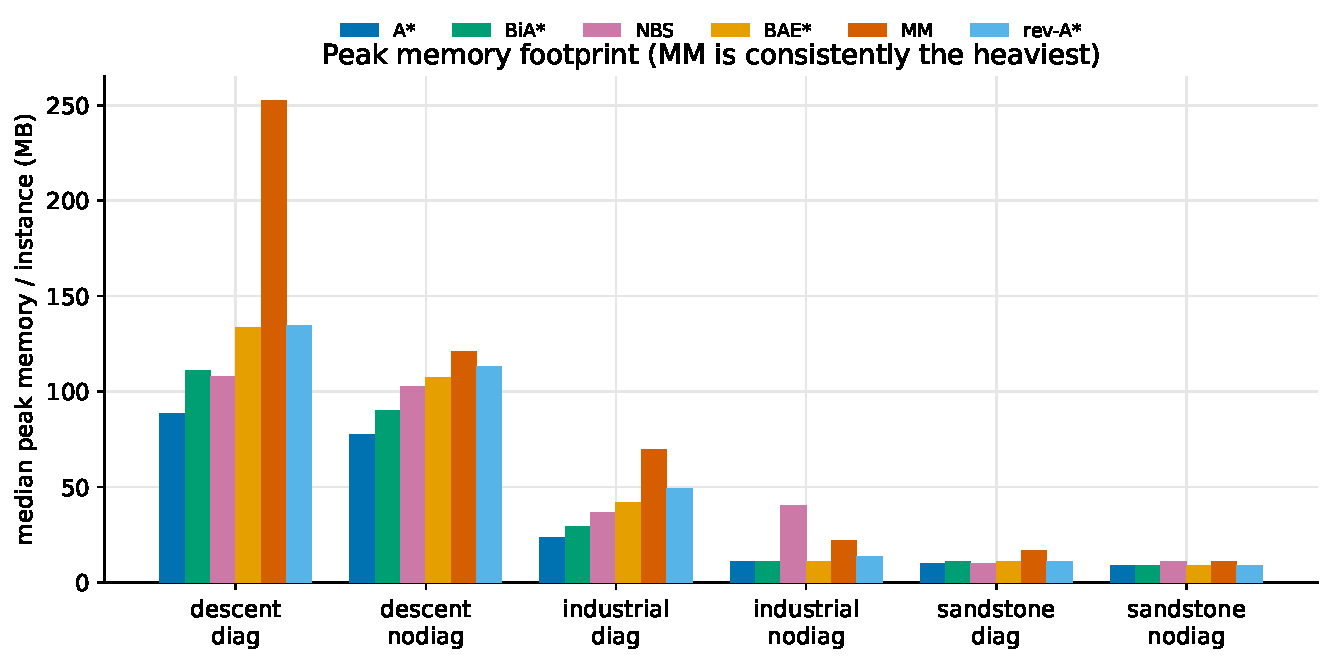
\includegraphics[width=\columnwidth]{figures/memory.pdf}
\caption{Peak memory footprint. MM is consistently the heaviest.}
\label{fig:mem}
\end{figure}

\subsection{(D) Direction}
Searching from the goal is not symmetric with searching from the start
(Figure~\ref{fig:asym}): reverse A* expands the most on plants but is competitive on
sandstone and descent. The asymmetry is domain-specific, matching the directional bias the
benchmark authors document in these maps \citep{brewer2018voxel,nobes2023voxel}.

\begin{figure}[t]
\centering
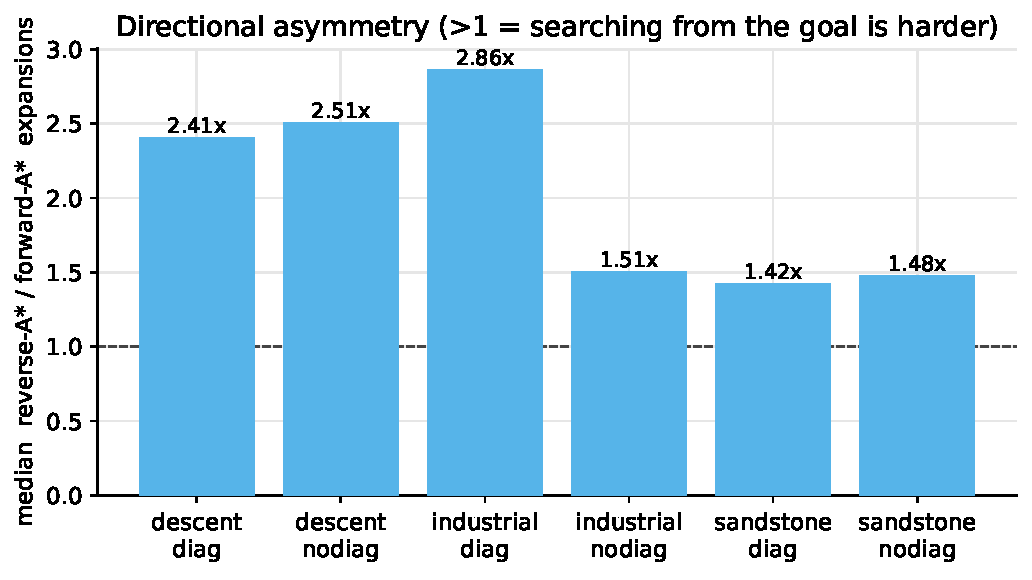
\includegraphics[width=0.86\columnwidth]{figures/directional_asymmetry.pdf}
\caption{Median reverse-A* / forward-A* expansions ($>1$: searching from the goal is harder).}
\label{fig:asym}
\end{figure}

\subsection{(E) The heuristic-strength crossover}
The central question---when bidirectional search becomes worthwhile---is answered by
weakening the heuristic (Table~\ref{tab:xover}, Figure~\ref{fig:xover}). At full strength A*
is best by a wide margin; as $w\to0$ it degrades fastest and \textbf{MM, then BAE*, overtake
it}, exactly the regime the theory predicts \citep{alcazar2020unifying,siag2025bridging}. The
nuance is that specifically the meet-in-the-middle (MM) and error-exploiting (BAE*) methods
cross over; plain BiA* and NBS do not.

\begin{table}[t]
\centering\small
\begin{tabular}{lccccc}
\hline
$w$ (weaker $\rightarrow$) & A* & MM & BAE* & BiA* & NBS \\
\hline
1.00 (full) & \textbf{801} & 19\,613 & 17\,218 & 1\,597 & 7\,395 \\
0.60 & 215\,578 & \textbf{79\,753} & 132\,233 & 306\,903 & 297\,017 \\
0.40 & 314\,929 & (timeout) & \textbf{110\,784} & 286\,395 & 211\,124 \\
\hline
\end{tabular}
\caption{Median expansions as the heuristic weakens (plant01).}
\label{tab:xover}
\end{table}

\begin{figure}[t]
\centering

\includegraphics[width=0.9\columnwidth]{figures/crossover.pdf}
\caption{Expansions vs.\ heuristic weight. A* goes from best to worst as $w\to0$; MM and
BAE* overtake it.}
\label{fig:xover}
\end{figure}

\subsection{Summary}
GBFS is not cost-optimal and is excluded from the floor comparison: it expands far fewer
nodes but returns longer paths---a speed/quality trade-off on a different axis. Overall,
across all three voxel domains, a strong consistent heuristic already puts A* at the
must-expand floor, so bidirectional search cannot help and in fact costs 2--5$\times$ more
work, more time, and more memory---MM most of all. The bidirectional advantage appears only
once the heuristic is weakened, and then only for the meet-in-the-middle and error-based
methods. This is precisely the theory-versus-practice gap the study set out to measure.

\section{Conclusions and Summary}
% Short: thesis and whether goals were met; contribution; limitations; future work.

\section{Code}
% Required by the guidelines.
\url{https://github.com/shpigelgi/final-project-voxel-bidirectional-search}

% \nocite{*}  % uncomment to list every reference before you cite them
% aaai2027.sty already sets the bibliography style; do NOT add \bibliographystyle.
\bibliography{references}

% ---- AAAI Reproducibility Checklist ----
% ReproducibilityChecklist.tex (in this folder) compiles on its own into a 2-page
% PDF (fill in the answers there). AAAI's camera-ready rule is one .tex per file,
% so submit the checklist as its own PDF rather than \input-ing it here. To fold it
% into this file instead, define the guard first and input it before \end{document}:
%   \def\isChecklistMainFile{}\input{ReproducibilityChecklist}

\end{document}
